\section{Introduction}
In this chapter, I aim to study the genetic toggle switch experimentally.  This chapter is organised as follows: In the first section I provide an overview of the circuit used and then outline the methods used for the experiments carried out. In the subsequent section I investigate the effect that the switch has on the growth rate of the bacteria. Then I examine the concentrations of the inducers and the time needed to flip the switch. 


\section{Flow cytometry and model fitting}

Flow cytometry detects the fluorescent intensity levels in individual cells. It can also provide physical information about the size and granularity of a cell via the forward and side scattering respectively. An overview of flow cytometry is shown in Figure~\ref{fig:flow_overv}. A laser excites the fluorochrome present in the bacterial cells. The fluorochromes emit a signal that is detected by channels in the optics. The signals are then all collected and analysed. A sample typically consists single cell measurements of $10^4$-$10^5$ cells. %Typically the cell populations are separated from the noise in the experiment via expert manual gating. Advances in flow cytometry technology has increased both the number of the dimensions of the datasets and the number of samples obtained, thus promoting the development for automated methods~\autocite{Johnsson:2016fd, Chen:2015bp, ONeill:2013cs}.



\begin{figure*}[tb]
	\begin{center}
		\includegraphics[scale=0.9]{chapterABCFlow/images/flow-overview.png}
	\caption[LoF caption]{\label{fig:flow_overv}: Flow cytometry. A laser excites the fluorescent proteins present in each cell. The cytometer has up to 4 lasers, violet (V), red (R), yellow (Y) and blue (B). The detectors in the optics, FL1-4 pick up the signals. The cytometer also picks up size and granularity information via the forward scatter (FSC) and side scatter (SSC) detectors. }
	\end{center}
\end{figure*}


Flow cytometry is used in synthetic biology, among others, for BioBrick characterisation~\autocite{Kelly:2009bj}, enzyme screening~\autocite{Choi:2014gb} and industrial  bioprocesses~\autocite{Diaz:2010kw}. Flow cytometry is a powerful tool for synthetic biology as it can measure multiple parameters in single cells, and process up to 35,000 cells sec\textsuperscript{-1}~\autocite{Anonymous:2015tj}. 

A drawback of flow cytometry is that the fluorescence intensity per cell is measured rather than number of proteins. Measuring absolute numbers of protein would be ideal for model fitting, but this type of biological data cannot be directly measured~\autocite{Kelwick:2014iy}. Standardization of experimental methods in flow cytometry has aided the effort to convert relative measurements, like fluorescence intensity, to absolute measurements, like GFP cell\textsuperscript{-1} s\textsuperscript{-1}~\autocite{Kelly:2009bj, Kelwick:2014iy}. 

In this chapter, I developed ABC-Flow, a method to fit computational models to experimental flow cytometry data. ABC-Flow approaches the problem of absolute protein numbers by converting the model output of GFP cell\textsuperscript{-1} s\textsuperscript{-1} to relative fluorescence intensity. ABC-Flow is a python package that uses Bayesian statistics to fit the parameters of a given model to flow cytometry time course data. The algorithm and its usage is described in Section~\ref{sec:abcflow-meth}.

%Progress has been made in the development of computational tools for the automated analysis of flow cytometry data from the field of computational immunology~\autocite{Saeys:2016im}. These tools are used for automated gating~\autocite{Lo:2008it, Aghaeepour:2011fv, Johnsson:2016fd} as well as modelling of cellular processes over time~\autocite{Bendall:2014hs, Bagwell:2015gp}. These methods are used to track different subpopulations over time, in order to follow the underlying developmental trajectory~\autocite{Saeys:2016im} and thus cannot be applied to experiments involving uniform cell populations. 


% is necessary as flow cytometry measures the intensity of the fluorescent proteins of interest in each cell.

 %On the other hand, when simulating a model, the output is measured in number of fluorescent proteins. It is thus essential to convert the simulated signal to the same format as the data, thus convert the number of fluorescent proteins to intensity measures. 

\section{Circuit overview}

The toggle switch plasmid I used here was provided by ~\textcite{Litcofsky:2012gr}. All the switch components were contained in one plasmid, pKDL071. An overview of the plasmid is shown in Figure~\ref{fig:pKDL071map}A and the sequence given in Appendix (XXX). The circuit consists of two promoters, Ptrc2 and PLtetO-1~\autocite{Lutz:1997ti}. Ptrc2 is a constitutive promoter, repressible by LacI. PLtetO-1 is also a constitutive promoter, repressible by TetR, as shown in Figure~\ref{fig:pKDL071map}B. mCherry~\autocite{Shaner:2004vy} and \acrshort{gfp}~\autocite{SHIMOMURA:1962va} are fluorescent proteins, that were added under the control of the same promoters as the repressors, and thus reflect the levels of TetR and LacI in the system. The plasmid contains kanamycin antibiotic resistance and is high copy (ColE1 origin of replication).

This system is capable of two states, GFP high and mCherry high. When \acrshort{iptg} is added to the system, it represses the repression of TetR and mCherry and thus the cells end up in the mCherry high state. When \acrshort{atc} is added to the system, it represses the repression of LacI and GFP and thus the cells end up in the GFP high state. If no inducer is added to the system it will randomly go to the GFP high or mCherry high states.

\begin{figure*}[tb]
	\begin{center}
		\includegraphics[scale=0.55]{chapterCharacterisation/images/pKDL071_overview.png}
	\caption[LoF caption]{\label{fig:pKDL071map}: The genetic toggle switch circuit used in this chapter. (A) The plasmid map of pKDL071, the plasmid containing the genetic toggle switch used in~\textcite{Litcofsky:2012gr} (B) The interactions between each element of the circuit.}
	\end{center}
\end{figure*}
\clearpage


\section{Methods}

The toggle switch plasmid was provided by the James J Collins lab in the form of a stab culture in \textit{E. coli} K-12 MG1655.

\subsection{\textit{Escherichia coli} culturing conditions}
\label{sec:overnigh_cult}

\acrfull{lb} was made by diluting \acrshort{lb} in deionized water to a concentration of \SI{25}{\gram\per\liter} and subsequently autoclaved. \acrshort{lb} agar plates were made by adding bacteriological agar to the above solution to a concentration of \SI{45}{\milli\gram\per\milli\liter} before autoclaving. The solution was then cooled down to \SI{55}{\celsius} using a water bath. If antibiotic was required it was added to the correct concentration to the cooled solution. The solution was then aliquoted to plates and left to solidify in room temperature. The plates were stored in the fridge for up to 1 month. 

Overnight cultures were made by picking a single colony from a static culture in an agar plate. Each colony was placed in \SI{15}{\milli\liter} Falcon tubes (Fisher Scientific, MA, U.S.A) with \SI{5}{\milli\liter} \acrshort{lb} with kanamycin antibiotic at a concentration of \SI{50}{\micro\gram\per\milli\liter}. The tubes were then screwed loosely and taped securely in order to allow for aeration. The falcon tubes were put in an incubator at \SI{37}{\celsius} with orbital shaking at \SI{200} rpm for 12-16 hours. 

\subsection{Inducers}

Anhydrotetracycline (ATc) solution was made by diluting \acrshort{atc} from Cayman Chemical Company in \SI{100}\% ethanol to a concentration of \SI{1}{\milli\gram\per\milli\liter}. \acrfull{iptg} solution was made by dissolving \acrshort{iptg} in deionized water to a concentration of \SI{1}{\molar}. The solution was sterilised by passing the solution through a \SI{0.22}{\micro\meter} syringe filter. Both inducers were stored in \SI{1}{\milli\liter} aliquots at \SI{-20}{\celsius}. 

\subsection{Glycerol stock preparation}
\label{sec:glycerol_stock}
To preserve the transformed cultures long-term glycerol stocks were made. \SI{5}{\milli\liter} \acrshort{lb} and Kanamycin overnight cultures were made as described in Section~\ref{sec:overnigh_cult}. The cultures were kept on ice and \SI{70}\% glycerol was added to the cultures in a ratio of glycerol to culture of 1:7. These were aliquoted into cryovials and transferred to a \SI{-80}{\celsius} freezer for long-term storage.


\subsection{Revival}
For subsequent revival of the frozen cultures, a \SI{1.5}{\milli\liter} eppendorf tube was removed from the \SI{-80}{\celsius} freezer and put on ice. Small amount was streaked onto an agar plate containing \acrshort{lb} and kanamycin. The plates were stored in an incubator at \SI{37}{\celsius} overnight. Then the plates were sealed using parafilm and stored at \SI{4}{\celsius} for up to two weeks. 


\subsection{Plasmid construction}

I constructed two plasmids in order to use them for the flow cytometry experiments. The first plasmid, pSEVA281G contains the promoter PLtetO-1 and \acrshort{gfp} and the other, pSEVA281C, contains the promoter Ptrc2 and mCherry from PKDL071, shown in Figure~\ref{fig:psevas}. These two plasmids were used to determine the appropriate voltages for the lasers that excite \acrshort{gfp} and mCherry.

pSEVA281G was constructed by digesting pKDL071 and pSEVA281 using the protocol outlined in Section~\ref{sec:digest}. pSEVA281 is a plasmid backbone containing kanamycin resistance, a high copy origin of replication and a multiple cloning site. The digested fragments were isolated using gel purification (Section~\ref{sec:gel_electr}) and then ligated the isolated fragments (Section~\ref{sec:ligation}). \textit{Escherichia coli} Dh5\textalpha{} was then transformed with each plasmid (Section~\ref{sec:transfection}). pSEVA281C was constructed via \acrshort{pcr} cloning. \acrshort{pcr} was carried out using the pKDL071 plasmid as a template \acrshort{dna} using the protocol outlined in Section~\ref{sec:pcr}. Primers were chosen so that Ptrc2 and mCherry were copied and a Hind\RNum{3} restriction enzyme recognition sequence added to the fragment. The primers are listed in Appendix (XXX). The amplified \acrshort{dna} was purified using the Qiagen PCR cleanup kit (Qiagen, Crawley, U.K) and then carried out the rest of the cloning procedure as per plasmid pSEVA281G.

Following construction, each plasmid was isolated using the QIAprep Spin Miniprep Kit (Qiagen, Crawley, U.K). Plasmid concentration was determined using the Thermo Scientific NanoDrop 1000 Spectrophotometer (Fisher Scientific, MA, U.S.A).

\begin{figure*}[t]
	\begin{center}
		\includegraphics[width=\textwidth]{chapterCharacterisation/images/plasmids_constructed.png}
		\caption[LoF caption]{\label{fig:psevas}: The plasmids used to calibrate GFP and mCherry fluorescence. (A) pSEVA281G plasmid map (B) pSEVA281C plasmid map.  }
	\end{center}
\end{figure*}

\subsubsection{Polymerase Chain Reaction}
\label{sec:pcr}
In order to amplify DNA and add the restriction enzyme sites required, a \acrfull{pcr} reaction was carried out with mutagenic primers. A list of primers can be found in Appendix (XXX). Q5\textsuperscript{\textregistered} DNA Polymerase (NEB, MA, U.S.A) was used with its associated buffer, \acrshort{dntp} and Q5\textsuperscript{\textregistered} enhancer, as specified in Table~\ref{tab:pcr_rec}. \acrshort{pcr} reactions were run in a T100\textsuperscript{TM} thermal cycler (Bio-Rad Laboratories, Inc., UK) as per the Q5\textsuperscript{\textregistered} recommendations, and as outlined in Tables~\ref{tab:pcr_rec} and ~\ref{tab:pcr_sched}.

\begin{table}[H]
\centering
\caption{\acrshort{pcr} recipe}
\label{tab:pcr_rec}
\begin{tabular}{@{}ccc@{}}
\toprule
Reagent           & Final concentration & \SI{50}{\micro\liter} reaction \\ \midrule
Q5\textsuperscript{\textregistered} buffer 5X      & 1X                  & \SI{10}{\micro\liter}          \\
\acrshort{dntp}             & \SI{200}{\milli\molar} each          & \SI{1}{\micro\liter}           \\
Forward primer    & \SI{0.5}{\micro\molar}               & \SI{2.5}{\micro\liter}         \\
Reverse primer    & \SI{0.5}{\micro\molar}               & \SI{2.5}{\micro\liter}         \\
Template DNA      & \SI{2}{\micro\gram}/\SI{50}{\micro\liter}                 & -             \\
Q5\textsuperscript{\textregistered} \acrshort{dna} polymerase & \SI{0.02}{\unit\per\micro\liter}            & \SI{0.5}{\micro\liter}         \\
Q5\textsuperscript{\textregistered} enhancer       & 1X                  & \SI{10}{\milli\liter}          \\
\ce{H2O}               & -                   & to \SI{50}{\micro\liter}       \\ \bottomrule
\end{tabular}
\end{table}


\begin{table}[H]
\centering
\caption{Thermocycling conditions}
\label{tab:pcr_sched}
\begin{tabular}{@{}cccc@{}}
\toprule
Step            & Cycles              & Temperature           & Time                 \\ \midrule
Initiation      & 1                   & \SI{98}{\celsius} & \SI{30}{\second} \\
Denaturation    & \multirow{3}{*}{30} & \SI{98}{\celsius} & \SI{10}{\second} \\
Annealing        &                     & \SI{72}{\celsius} & \SI{20}{\second} \\
Extension       &                     & \SI{72}{\celsius} & \SI{2}{\minute}  \\
Final extension & 1                   & \SI{72}{\celsius} & \SI{2}{\minute}  \\
Hold            & 1                   & \SI{4}{\celsius}  & \infty            \\ \bottomrule  
\end{tabular}
\end{table}

\subsubsection{Digestion}
\label{sec:digest}

All enzymes, buffers and \acrfull{bsa} were supplied by NEB. Digestion controls were carried out by adding \ce{H2O} instead of \acrshort{dna} in the digestion reaction. Additionally, during agarose gel electrophoresis uncut plasmid was run alongside the digested plasmid in order to detect the difference. 

\SI{2}{\micro\gram} digests were set up by mixing the plasmid with \SI{0.5}{\micro\liter} of each restriction enzyme, \SI{3}{\micro\liter} 10x buffer and \SI{3}{\micro\liter} 10x \acrshort{bsa}. \ce{H2O} was added to make the reaction to \SI{20}{\micro\liter}. The recipe used is shown in Table~\ref{tab:digestion}. The reactions were placed in an incubator at \SI{37}{\celsius} for 4 hours. Finally, the solutions were analysed using agarose gel electrophoresis (Section~\ref{sec:gel_electr}).


\begin{table}[htbp]
\centering
\caption{Digestion recipe}
\label{tab:digestion}
\begin{tabular}{@{}cccc@{}}
\toprule
Reagent   & Volume  &  &  \\ \midrule
Pst\RNum{1}&                \SI{0.5}{\micro\liter}     &  &  \\
Hind\RNum{3} &                \SI{0.5}{\micro\liter}     &  &  \\
NEB Buffer 2.1        & \SI{2}{\micro\liter}       &  &  \\
BSA            & \SI{0.2}{\micro\liter}     &  &  \\
\acrshort{dna}              & \SI{1}{\micro\gram}       &  &  \\
\ce{H2O}           & to \SI{20}{\micro\liter} &  &  \\ \bottomrule
\end{tabular}
\end{table}


\subsubsection{Agarose gel electrophoresis}
\label{sec:gel_electr}
To make a 0.8\% agarose gel, \SI{0.4}{\gram} agarose were diluted in \SI{50}{\milli\liter} 1X TAE buffer. It was further dissolved by microwaving for 1-3 minutes. The solution was left to cool for 5 minutes and then \SI{1.5}{\micro\liter} gel red were added. Gel trays were prepared by putting the well comb in place and taping the ends shut. The solution wast then poured into the prepared gel trays and left to solidify for 20-30 minutes at room temperature.

Agarose gel electrophoresis was carried out by placing the poured gels into the gel tanks. The tank was then flooded with 1X TAE buffer. The \acrshort{dna} was prepared to be analysed by adding \SI{4}{\micro\liter} loading dye to \SI{20}{\micro\liter} sample. A negative control was used with \ce{H2O} instead of sample. The \acrshort{dna} ladder of choice was prepared by adding \SI{1}{\micro\liter} \ce{H2O} and \SI{1}{\micro\liter} dye to \SI{2}{\micro\liter} ladder. Each sample was added to a well by pipetting. The agarose gel was ran at \SI{90}{\volt} until the dye was 80\% of the way down the gel, approximately 1 hour.

To purify the fragments from the agarose gel, the gel was placed in a UV box. Using a sterile razor blade, the desired fragment was cut out and placed in a clean eppendorf tube. The \acrshort{dna} was isolated from the gel using the QIAquick Gel Extraction Kit.

\subsubsection{Ligation}
\label{sec:ligation}
A ratio of 3:1 of insert to recipient plasmid was used, \SI{1}{\micro\liter} T4\textsuperscript{\textregistered}  DNA ligase (NEB, MA, U.S.A) and \SI{2}{\micro\liter} ligase buffer. \ce{H2O} was added to make the reaction up to \SI{20}{\micro\liter}. The controls used for each ligation reaction, are shown in Table~\ref{tab:lig-contr}. Control 1 is used to detect competent cell viability, control 2 background due to uncut vector, control 3 contamination and control 4 vector re-circularization.  

The ligation reactions were placed at \SI{4}{\celsius} for 12 hours. The reactions were then placed at \SI{65}{\celsius} for 10 minutes to heat inactivate the T4 DNA ligase enzyme. A transformation was then carried out as per Section~\ref{sec:transfection}.

\begin{table}[htbp]
\centering
\caption{Ligation controls}
\label{tab:lig-contr}
\begin{tabular}{@{}ccccc@{}}
\toprule
       & Control 1 & Control 2 & Control 3 & Control 4 \\ \midrule
Vector &  Uncut    & \cmark    & \cmark    & \xmark    \\
Insert &  \xmark    & \xmark    & \xmark    & \cmark    \\
Buffer &  \cmark    & \cmark    & \cmark    & \cmark    \\
\ce{H2O}    & \cmark    & \cmark    & \cmark    & \cmark    \\
Ligase &  \xmark    & \xmark    & \cmark    & \cmark    \\ \bottomrule
\end{tabular}
\end{table}
\subsubsection{Transformation}
\label{sec:transfection}
Thermocompetent \textit{E.coli} Dh5\textalpha was transformed with the constructed plasmids. Each ligation reaction was added to \SI{50}{\micro\liter} of thawed competent cells. The cells were subsequently kept on ice for 30 minutes, then placed at a \SI{42}{\celsius} water bath for \SI{45}{\second}. The cells were then placed back on ice for 15 minutes. Then \SI{500}{\micro\liter} of Super Optimal broth with Catabolite repression (SOC) were added to each ligation and placed in a \SI{37}{\celsius} shaking incubator for 3 hours. \SI{500}{\micro\liter} and \SI{50}{\micro\liter} were subsequently pipetted of each ligation onto petri dishes with LB agar and the appropriate antibiotic. The plates were incubated at \SI{37}{\celsius} for 12-16 hours. Two controls were used for the transfection protocol, a positive control with no antibiotic in the LB agar and non-transfected cells and a negative control of non-transformed cells and LB agar with antibiotic. These ensure that the cells are viable and not contaminated respectively. 

Finally, the number of colonies were counted on each plate. Individual colonies were then selected from each transfection and grew each separately in \SI{5}{\milli\liter} LB medium for 12-16 hours at \SI{37}{\celsius}, 200 rpm. Glycerol stocks were then prepared from each culture, as per Section~\ref{sec:glycerol_stock}.



\subsubsection{Colony \acrshort{pcr}}

In order to determine if the fragment was successfully inserted into the vector \acrshort{dna} plasmid, diagnostic colony \acrshort{pcr} was then carried out. Primers were designed that amplified the multiple cloning site of the vector \acrshort{dna} plasmid. These can be found in Appendix (XXX). A \acrshort{pcr} master mix was made for the number of colonies to be amplified, 32, with an added 10\% to account for pipetting error. GoTaq\textsuperscript{\textregistered} Flexi \acrshort{dna} polymerase (Promega Corp., WI, U.S.A.) was used with its associated buffer, \acrshort{dntp} and \ce{MgCl2}and \ce{H2O}. The recipe for the master mix is shown in Table~\ref{tab:pcr_mastex_mix}.

\begin{table}[htbp]
\centering
\caption{Colony \acrshort{pcr} master mix recipe}
\label{tab:pcr_mastex_mix}
\begin{tabular}{@{}ccc@{}}
\toprule
Reagent           & Final concentration & Master mix \\ \midrule
GoTaq\textsuperscript{\textregistered} green Flexi buffer      & 1X                  & \SI{141}{\micro\liter}          \\
\acrshort{dntp}             & \SI{200}{\milli\molar} each          & \SI{14.1}{\micro\liter}           \\
Forward primer    & \SI{0.5}{\micro\molar}               & \SI{1.4}{\micro\liter}         \\
Reverse primer    & \SI{0.5}{\micro\molar}               & \SI{1.4}{\micro\liter}         \\
GoTaq\textsuperscript{\textregistered} Flexi polymerase & \SI{0.02}{\unit\per\micro\liter}            & \SI{3.5}{\micro\liter}         \\
\ce{MgCl2}       & 1X                  & \SI{42.2}{\micro\liter}          \\
\ce{H2O}               &     -               & \SI{465}{\micro\liter}       \\ \bottomrule
\end{tabular}
\end{table}

\SI{19}{\micro\liter} were then added from the master mix to each \acrshort{pcr} tube. Each of the colonies was then lifted from the transformation from the agar plate using a \SI{20}{\micro\liter} pipette tip and added it to a \acrshort{pcr} mix by mixing. The pipette tip was subsequently used to make a scratch into a clean agar plate, and labelled it. A \acrshort{pcr} was then carried out according to GoTaq\textsuperscript{\textregistered} Flexi polymerase recommendations, and as shown in Table~\ref{tab:pcr_sched_col}.

\begin{table}[H]
\centering
\caption{Thermocycling conditions for colony \acrshort{pcr}}
\label{tab:pcr_sched_col}
\begin{tabular}{@{}cccc@{}}
\toprule
Step            & Cycles              & Temperature           & Time                 \\ \midrule
Cell lysis      & 1                   & \SI{95}{\celsius} & \SI{10} minutes \\

Denaturation    & \multirow{3}{*}{35} & \SI{95}{\celsius} & \SI{30}{\second} \\
Annealing        &                     & \SI{50}{\celsius} & \SI{1} minute \\
Extension       &                     & \SI{72}{\celsius} & \SI{1}{\minute}  \\

Final extension & 1                   & \SI{72}{\celsius} & \SI{5}{\minute}  \\
Hold            & 1                   & \SI{4}{\celsius}  & \infty            \\ \bottomrule  
\end{tabular}
\end{table}

Finally a diagnostic agarose gel electrophoresis was carried out as outlined in Section~\ref{sec:gel_electr}.

\subsubsection{Sequencing}
In order to confirm plasmid identity, all plasmids were sequenced using Source Bioscience, Cambridge UK. \SI{10}{\micro\liter}  of each plasmid DNA were submitted at a minimum of \SI{100}{\nano\gram\per\micro\liter} as per the requirements. Primer sequences were also submitted and manufactured by Source Bioscience. Primers can be found in Appendix (XXX). 

\subsection{Growth rate measurement}
\label{sec:growth_meth}
Plate reader analysis was carried out in order to measure the growth of \textit{E.coli} over time. Overnight cultures were made using the method shown in Section~\ref{sec:overnigh_cult}. Overnight cultures were then diluted by a 1:1000 ratio into a \SI{5}{\milli\liter} \acrshort{lb} + kanamycin solution. The diluted cultures were grown at \SI{37}{\celsius} with shaking at 200rpm for 1 hour. These cultures were then further diluted by a 1:100 ratio. \SI{200}{\ul} aliquots of the dilutions were then transferred to a clear bottom, black-walled 96-well plate. Wells with only LB and kanamycin were also added in order to be used as blanks. The plate was then sealed using a gas permeable membrane and placed it in BMG FLUOstat OPTIMA plate reader to measure absorbance. The plate reader was set to a constant \SI{37}{\celsius}, with 30 seconds orbital shaking at \SI{150}rpm and \SI{4}{\milli\metre} shaking width every ten minutes. Absorbance was measured at \SI{540}{\nano\meter}. Data was exported as a CSV file and analysed using Python. 

\subsection{Flow cytometry}
Flow cytometry experiments were carried out in order to get fluorescent levels in single cells. Flow cytometry allows us to gather this information for thousands of single cells. Flow cytometry data was exported as FCS files and analysed using the R bioconductor packages flowCore~\autocite{flowCore:man}, flowViz~\autocite{flowViz:man} and Ggplot2~\autocite{ggplot2:bk}. 

\subsubsection{Concentration assays}
\label{sec:flo_conc}
Concentration assays were carried out in order to determine the concentration of each inducer (\acrshort{atc} and \acrshort{iptg}) at which the switch flips.  Separate overnight cultures were prepared as per Section~\ref{sec:overnigh_cult} with added \acrshort{iptg} at a concentration of \SI{1}{\milli\molar} or added \acrshort{atc} at a concentration of \SI{100}{\nano\gram\per\milli\liter}~\autocite{Litcofsky:2012gr}. The cultures were then diluted by 1:1000 into fresh \acrshort{lb} medium with varying concentrations of the opposite inducer than what the cells were grown in overnight. The concentrations used are shown in Table~\ref{tab:flow_conc}. For each concentration. three replicates cultures were made.


\begin{table}[htbp]
\centering
\caption{Concentrations used for flow cytometry assay}
\label{tab:flow_conc}
\begin{tabular}{@{}cc@{}}
\toprule
\acrshort{atc} (ng/ml)  & \acrshort{iptg} (M) \\ \midrule
0.05 & 1e-7 \\
0.06 & 6e-7 \\
0.07 & 1e-6 \\
0.08 & 6e-6 \\
0.09 & 1e-5 \\
0.1  & 1e-3 \\
1.0  & 0.1  \\ \bottomrule
\end{tabular}
\end{table}

The cultures were placed in an incubator at \SI{37}{\celsius}, 200rpm for 5 hours. The cultures were then placed in a centrifuge and spun at 13,000rpm for 5 minutes. The supernatant was discarded and replaced it with \SI{1}{\milli\liter} PBS solution. The BD LSRFortessa\textsuperscript{TM} cell analyzer (Becton, Dickinson and Company) was used at the St. Mary's Flow Cytometry Core Facility at Imperial College London  for flow cytometry analysis. \acrshort{gfp} was excited using the \SI{488}{\nano\meter} laser and detected using the 533/30 filter. mCherry was excited using the \SI{561}{\nano\meter} laser and detected using the 620/10 filter. Data was obtained at n=10000 events per experiment. 

\subsubsection{Time course assays}
\label{sec:flo_time}
Time course assays were carried out to measure the time it takes for the switch to flip to each state. Separate overnight cultures of pKDL071 were prepared as per Section~\ref{sec:overnigh_cult} with added \acrshort{iptg} at a concentration of \SI{1}{\milli\molar} or added \acrshort{atc} at a concentration of \SI{100}{\nano\gram\per\milli\liter}~\autocite{Litcofsky:2012gr}. Overnight cultures of pSEVA281G and pSEVA281C were also made. The cultures were then diluted by a ratio of 1:1000 into fresh LB medium. Separate cultures for each time point were made, in triplicate. For cultures grown overnight in \acrshort{iptg}, \acrshort{atc} was added at a concentration of \SI{100}{\nano\gram\per\milli\liter} and for cultures grown overnight in \acrshort{atc}, \acrshort{iptg} was added at a concentration of \SI{1}{\milli\molar}. All cultures were placed at \SI{37}{\celsius}, 200rpm incubator. At 30 minutes, 1 hour and then every hour up to 6 hours flow cytometry was carried out for the corresponding cultures. Triplicates for each induction were removed from the incubator and placed in a centrifuge at 13, 000rpm for 10 minutes. The supernatant was discarded and replaced with \SI{1}{\milli\liter} PBS solution. These cultures were then analysed in an Attune\textsuperscript{TM} NxT Flow Cytometer (Thermo Fisher Scientific) at University College London. \acrshort{gfp} was excited using the \SI{488}{\nano\meter} laser and detected using the 533/30 filter. mCherry was excited using the \SI{561}{\nano\meter} laser and detected using the 620/10 filter. Data was obtained at n=10000 events per experiment. pSEVA281G and pSEVA281C cultures were used to set the laser voltages and pKDL071 cultures to detect the bacteria population.  

\subsection{ABC-Flow algorithm}
\label{sec:abcflow-meth}

The algorithm of ABC-Flow is based on the same ABC algorithm as ABC-SysBio and Stability Finder described in Sections (XXX), adapted to be used for flow cytometry data. The algorithm of ABC-Flow is outlined in Algorithm~\ref{alg:abc-flow}. The modified modules of the ABC algorithm are outlined in the sections that follow.

\begin{figure*}[htbp]
	\begin{center}
		\includegraphics[scale=0.7]{chapterABCFlow/images/abc-flow-overv.png}
		\caption[LoF caption]{\label{fig:abcflow-overv}: Overview of ABC-Flow. (A) ABC-Flow is used to fit models to experimental flow cytometry data. (B) The algorithm can be applied to 1D and 2D flow data. (C) ABC-Flow uses approximate bayesian computation.}
	\end{center}
\end{figure*}

The user provides an SBML model file and an input file to specify the information needed to run ABC-Flow, like the \epsilon schedule and the priors to the parameters. The user must also provide a data file containing the flow cytometry data to which the model will be fitted. The data files used here were generated from .fcs files, which is the standard output of flow cytometers using the R bioconductor packages flowCore~\autocite{flowCore:man}. ABC-Flow simulations are implemented on \acrshort{gpu}s.



\begin{algorithm}[htbp]

\caption{ABC-Flow}
\label{alg:abc-flow}
 \begin{algorithmic}[1]
 	\Statex
% \State Read input file
%	\If{ABC-Rejection}
% 		\State Sample from priors
% 		\State Simulate model
% 		\State Convert signal to intensity
% 		\State Measure distance to data
%		\State Reject particles if d $\textgreater$ $\epsilon$.
% 		\If{number of accepted particles == number of particles}
% 			\State Exit
% 		\Else
% 			\State Return to step 3.
% 		\EndIf
% 	\EndIf
 	
 	%\If{ABC-SMC}
	\State Initialise $\epsilon$ 
	\Let{population p}{1}
	\If{p $= 1$}
		\State Sample particles ($\theta$) from priors
		\Else
			\State Sample particles from previous population
			\State Perturb each particle by $\pm$ half the range of the previous population (j) to obtain new perturbed population (i).
	\EndIf
	\State Simulate model
	\State Convert signal to intensity: 
	\For{each particle}
		\For{each beta}
			\For{each timepoint}
				\For{each fluorescent protein}
					\State Intensity = N\bigg(signal\times$\mu$,  $\sqrt{(signal\times\sigma^2)}$\bigg)
	\EndFor				
	\EndFor	
	\EndFor	
	\EndFor	
	\State Measure distance to data
	\State Reject particles if d $\textgreater$ $\epsilon$.
    \State Calculate weight for each accepted $\theta$
	\State $w_{t}^{(i)} = \begin{cases} 1, & \mbox{if } p = 0 \\\frac{\pi(\theta_{t}^{(i)})}{\sum_{j=1}^N w_{t-1}^{(j)} K_{t}(\theta_{t-1}^{(j)}, \theta_{t}^{(i)})}, & \mbox{if } p \geq  0. \end{cases}$
	\State Normalise weights
	\State Repeat steps 3 - 15 until $\epsilon \leq \epsilon_T$	%EndIf
  \end{algorithmic}
\end{algorithm}

\clearpage
\subsubsection{Distance Calculations}

The distance in the 1D case was calculated using the Kolmogorov-Smirnov test~\autocite{Kolmogorov:1933}. The Kolmogorov-Smirnov test is a non-parametric statistic test that determines whether the two distribution functions differ. The KS distance between two distributions is equal to the largest distance between the empirical distribution functions of the two samples, as illustrated in Figure~\ref{fig:ks-dist} and Equation~\ref{eq:ks1d}.

\begin{align}
\label{eq:ks1d}
D_{n,n'}=\sup _{x}|F_{1,n}(x)-F_{2,n'}(x)|
\end{align}



\begin{figure*}[htbp]
\begin{center}
	\includegraphics[scale=0.5]{chapterABCFlow/images/ks-1d-overv.png}
			\caption[LoF caption]{\label{fig:ks-dist}:The Kolmogorov-Smirnov distance function used to calculate the distance between distributions in the 1D case.}
	\end{center}
\end{figure*}



%A grid is first defined, from the minimum to the maximum value in the dataset. A gaussian kernel is fit to the experimental and the simulated data, at each timepoint for the given grid. The distance between the two kernels is then defined by:

%\begin{align*}%
%	d = \sum_{i=xmin}^{xmax} (fD_i - fS_i)^2
%\end{align*}


For the 2D case the distance was calculated in a similar way, by using an adaptation of the Kolmogorov-Smirnov distance in higher dimensions~\autocite{Peacock:1983fa}.

%\begin{figure*}[htbp]
%	\begin{center}
%		\includegraphics[scale=0.8]{chapterABCFlow/images/KS-dist.png}
%		\caption[LoF caption]{\label{fig:ks-dist}:The Kolmogorov-Smirnov distance function used to calculate the distance between distributions in the 1D (A) and 2D (B) cases.}
%	\end{center}
%\end{figure*}
%\clearpage
\clearpage
\subsubsection{Intensity calculation}

The units of the result of the stochastic simulations is in the form of number of fluorescent proteins. On the other hand, flow cytometry data units are in the form of fluorescence intensity. For ABC-Flow, the simulation results are converted to intensity in order to be able to compare the data to the simulations. In order to do this two additional parameters are defined, intensity \textmu{} and intensity \textsigma{}, for each fluorescent protein used. To convert the number of fluorescent proteins to intensity, random samples are drawn from a normal distribution:

\begin{align}
	X\sim N\Big(nFP\times\mu, \sqrt{(nFP\times\sigma^2)}\Big), \label{eq:intens}
\end{align}
where nFP is the number of fluorescent proteins. 


These parameters are fitted to the data along with the model parameters.  

\begin{figure*}[htbp]
	\begin{center}
		\includegraphics[scale=0.6]{chapterABCFlow/images/intensity_calc.png}
		\caption[LoF caption]{\label{fig:intensity_calc}:Converting the number of fluorescent proteins to the intensity (iFP) is done by drawing from a normal distribution, as shown in Equation~\ref{eq:intens}.}
	\end{center}
\end{figure*}

\section{Results}
\subsection{Growth rate investigation}

I carried out a growth rate analysis to determine whether the \acrshort{atc} or \acrshort{iptg} added to pKDL071 or pSEVA281G \textit{E. coli} cultures affected the growth of the bacteria. Cultures were grown without any inducer overnight as described in Section~\ref{sec:growth_meth}. I ran assays for the cultures with and without added inducers. As can be seen in Figure~\ref{fig:growth_curve}, there is no difference between the conditions. The addition of either \acrshort{atc} or \acrshort{iptg} does not affect the growth rate of \textit{E. coli} K-12 MG1655. Additionally, \acrshort{atc} does not affect the growth rate of \textit{E. coli} Dh5\textalpha. Since the addition of \acrshort{atc} flips the switch to the GFP high state, and \acrshort{iptg} to the mCherry high state, we can also conclude that the growth rate of the chassis is not affected by which side of the switch is in the high state. The growth rate of \textit{E. coli} Dh5\textalpha was consistently lower than that of \textit{E. coli} K-12 MG1655.

\begin{figure*}[htbp]
	\begin{center}
		\includegraphics[scale=0.7]{chapterCharacterisation/images/growth_curves.pdf}
		\caption[LoF caption]{\label{fig:growth_curve}: Growth rate analysis of \textit{E. coli} K-12 MG1655 pKDL071 and \textit{E. coli} Dh5\textalpha pSEVA281G cultures with and without inducers. The inducers do not affect the growth of the bacteria. }
	\end{center}
\end{figure*}

\clearpage

\subsection{Toggle switch concentration assays}

Here I aim to identify the inducer concentration at which the pKDL071 toggle switch changes state. In order to do that I carry out a concentration assay using flow cytometry, as described in Section~\ref{sec:flo_conc}. As can be seen in Figure~\ref{fig:switch_concent2d1d}A, during \acrshort{atc} induction the switch flips to a GFP high state when \acrshort{atc} concentration is at \SI{0.09}{\nano\gram\per\milli\liter} or higher. We observe a bimodal distribution at concentrations \SI{0.07}{\nano\gram\per\milli\liter} and \SI{0.08}{\nano\gram\per\milli\liter}, which indicates that the switching has begun at these concentrations. Thats why part of the population has switched to the GFP high state but complete switching is not observed until the concentration of \acrshort{atc} is at \SI{0.09}{\nano\gram\per\milli\liter}. In the case of \acrshort{iptg} induction (Figure~\ref{fig:switch_concent2d1d}B) we find that the switch flips to the mCherry high state when the concentration of \acrshort{iptg} is higher or equal to 0.001M. A decrease in GFP fluorescence is also observed. We do not observe a bimodal distribution in this case. 

\begin{figure*}[htbp]
	\begin{center}
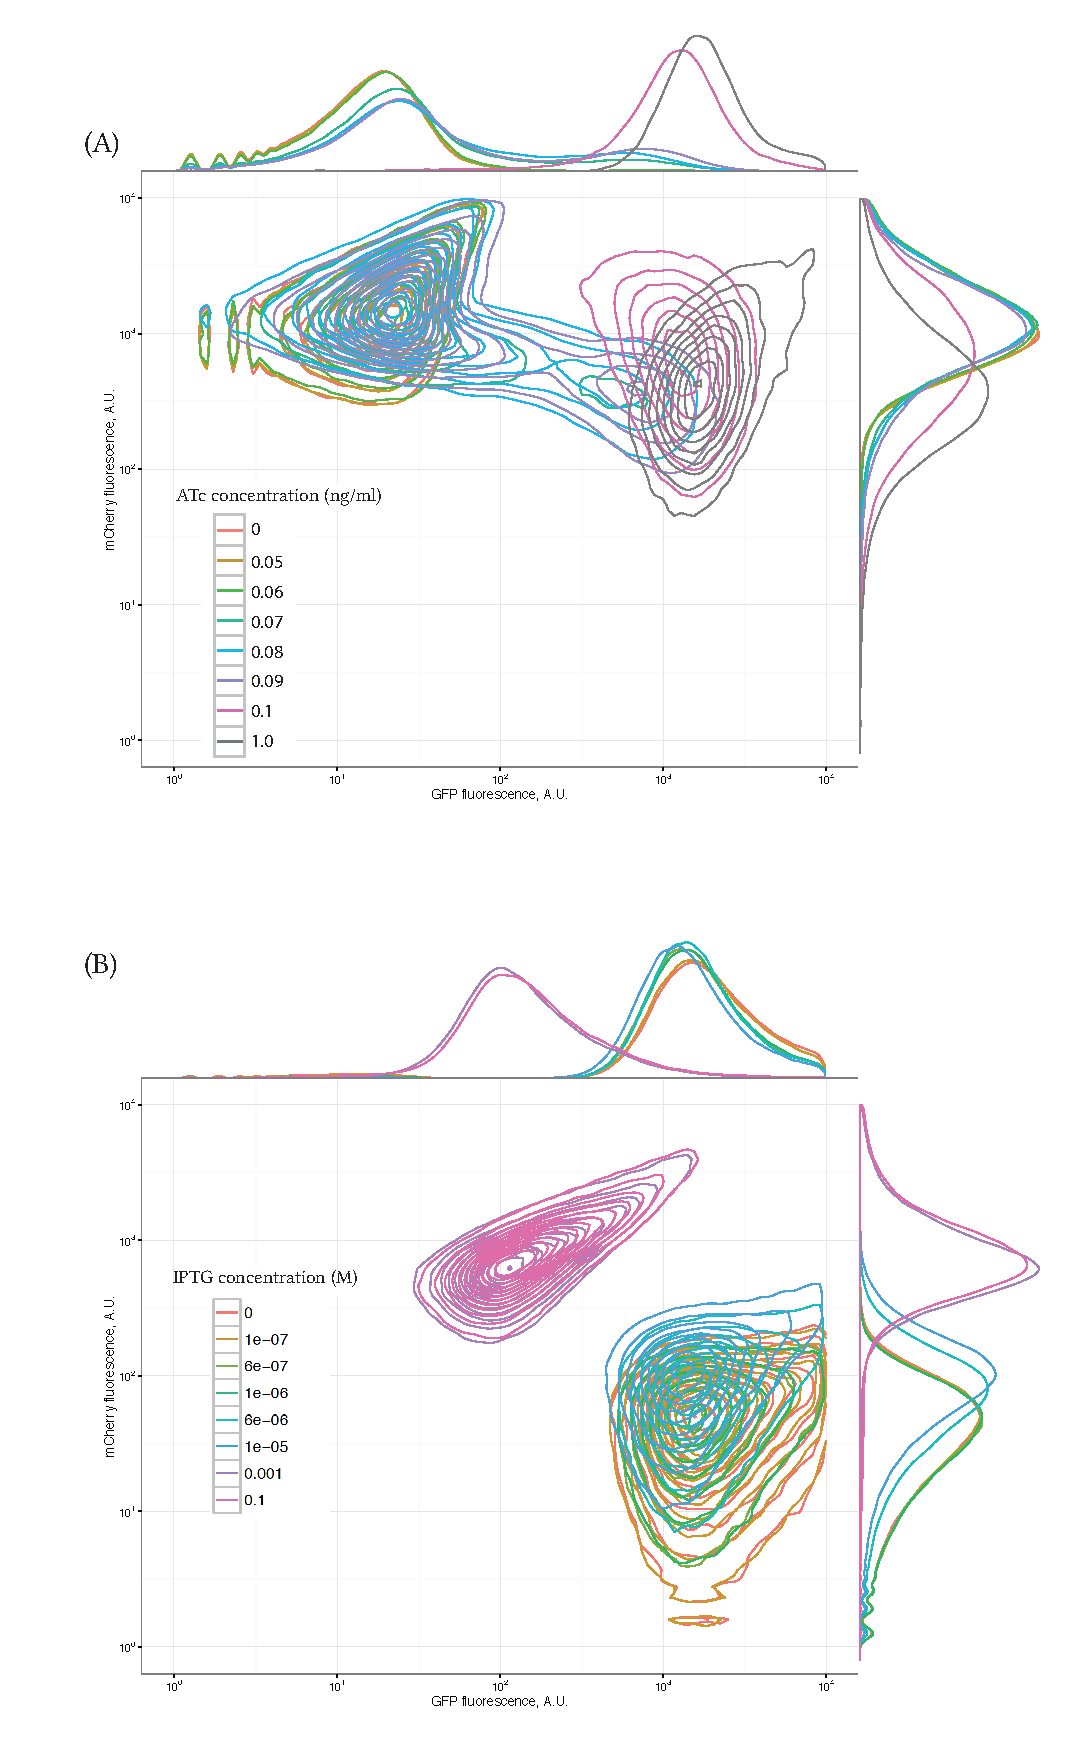
\includegraphics[scale=0.7]{chapterCharacterisation/images/pKDL071_concentrations_2d1d.png}
\caption[LoF caption]{\label{fig:switch_concent2d1d}: (A) \acrshort{atc} induction at various concentrations (B) \acrshort{iptg} induction at various concentrations. }
\end{center}
\end{figure*}
\clearpage

By taking into account the two induction curves of the switch turning to each high state, we can see the dynamic ranges of pKDL071 in \textit{E.coli}. We can see in Figure~\ref{fig:switch_concentrations_model} there is an approximately 100-fold change in fluorescent units during \acrshort{iptg} and \acrshort{atc} induction. 

 A Hill function was used to model the characterisation curves shown in Figure~\ref{fig:switch_concentrations_model}. The model used is the following:
 \begin{align}
 	F = Pmin + (Pmax - Pmin)\frac{\Big(\frac{[I]}{Kd}\Big)^n}{1+\Big(\frac{[I]}{Kd}\Big)^n},
 \end{align}
 
where F is the median fluorescent unit and [I] is the concentration of inducer. Pmin and Pmax are the minimum and maximum fluorescence respectively, and Kd and n are the dissociation constant, and Hill coefficient. I fit Hill function models using maximum likelihood estimation to the response curves. The values for parameters Pmin, Pmax, Kd, and n are 8, 1600, 0.1, 1.8 respectively for the \acrshort{atc} induction and 8, 700, 0.08, 2.5 for \acrshort{iptg} induction. 

\begin{figure*}[tb]
	\begin{center}
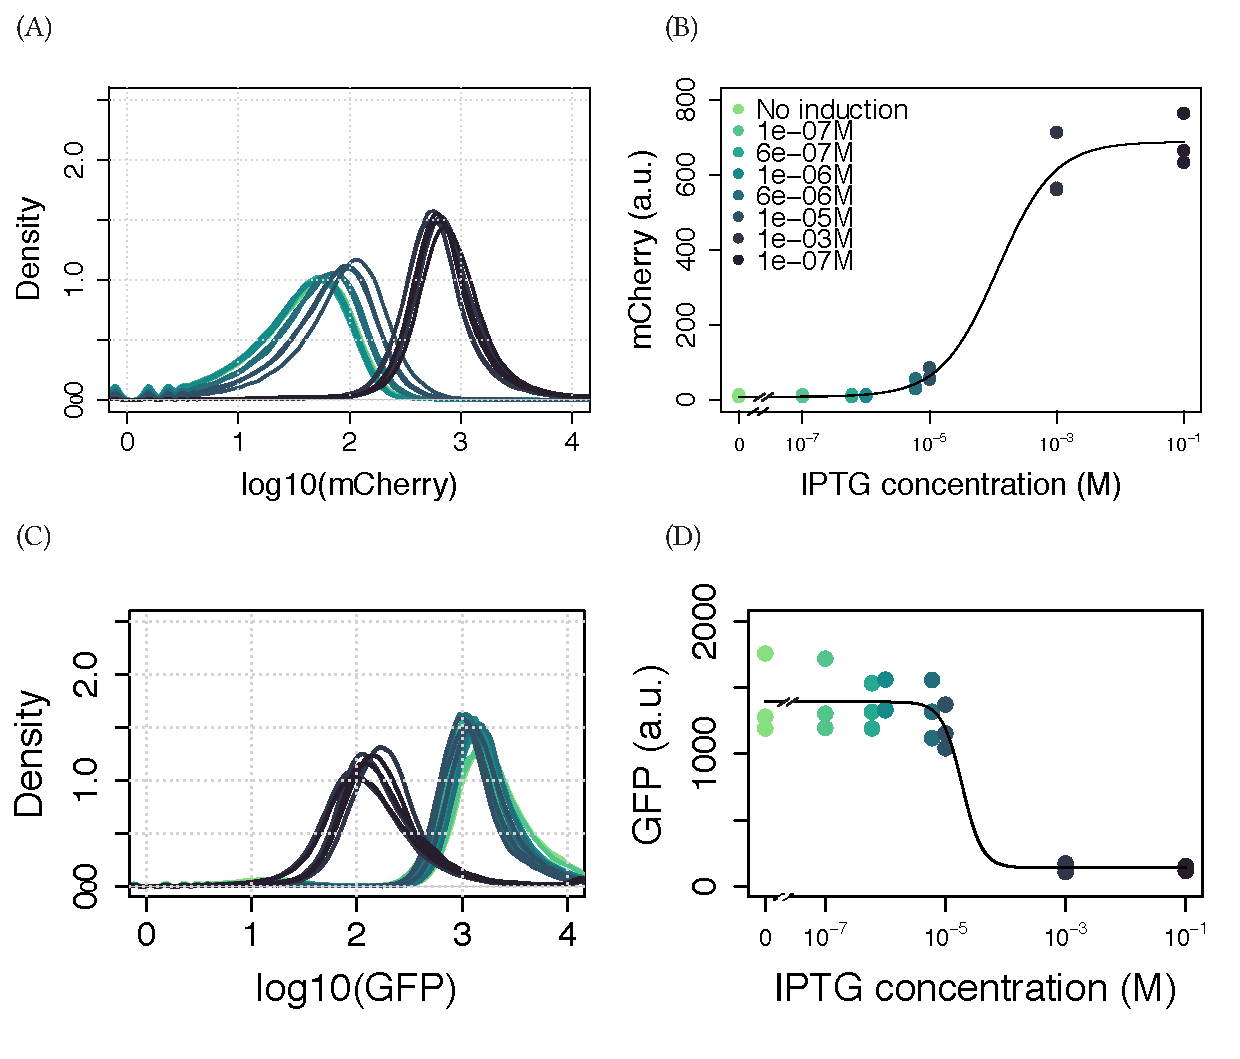
\includegraphics[width=\textwidth]{chapterCharacterisation/images/pKDL071_concentrations_model_fit.png}
\caption[LoF caption]{\label{fig:switch_concentrations_model}: (A, B) \acrshort{atc} induction of pKDL071. (C, D) \acrshort{iptg} induction of pKDL071.}
\end{center}
\end{figure*}


For the case of the \acrshort{atc} induction we observe a sharp switch between the GFP low to the GFP high state, as can be seen in the characterisation curve in Figure~\ref{fig:switch_concentrations_model}B. This is a clear indication of the bistability of this switch.

\clearpage





\subsection{Toggle switch time course assay}
\label{sec:ts_time}
I further analysed the pKDL071 toggle switch by investigating the time it takes for it to switch from one high state to the other. To do that I used the method outlined in Section~\ref{sec:flo_time}. I obtained separate time courses for the \acrshort{iptg} and \acrshort{atc} inductions. 

As can be seen in Figure~\ref{fig:switch_timecourse_atc} pKDL071 \acrshort{atc}  induction begins switching 1 hour after induction. Complete induction is seen at 6 hours. During the \acrshort{iptg} induction (Figure~\ref{fig:switch_timecourse_iptg}) we see a bimodal distribution at 4 hours, and induction is complete at 6 hours. We observe that during \acrshort{atc} induction there is an increase in \acrshort{gfp} fluorescence and a decrease in mCherry fluorescence, in the case of \acrshort{iptg} induction the increase in mCherry fluorescence is not as prominent. A decrease in GFP fluorescence is observed during \acrshort{iptg} induction. 

\begin{figure*}[tb]
	\begin{center}
\includegraphics[scale=0.7]{chapterCharacterisation/images/pKDL071_atc_time.png}
\caption[LoF caption]{\label{fig:switch_timecourse_atc}: \acrshort{atc} induction of pKDL071 over time}
\end{center}
\end{figure*}


\begin{figure*}[tb]
	\begin{center}
\includegraphics[scale=0.7]{chapterCharacterisation/images/pKDL071_iptg_time.png}
\caption[LoF caption]{\label{fig:switch_timecourse_iptg}: \acrshort{iptg} induction of pKDL071 over time}
\end{center}
\end{figure*}
\clearpage


%\begin{figure*}[tb]
%	\begin{center}
%\includegraphics[scale=0.5]{chapterCharacterisation/images/atc_timecourse.png}
%\caption[LoF caption]{\label{fig:atc_timecourse}: \acrshort{atc} induction of pKDL071 over time}
%\end{center}
%\end{figure*}
%
%\begin{figure*}[tb]
%	\begin{center}
%\includegraphics[scale=0.5]{chapterCharacterisation/images/iptg_timcourse.png}
%\caption[LoF caption]{\label{fig:iptg_timecourse}: \acrshort{iptg} induction of pKDL071 over time}
%\end{center}
%\end{figure*}
%\clearpage


